%%%%%%%%%%%%%%%%%%%%%%%%%%%%%%%%%%%%%%%%%
% Maggi Memoir Thesis
% XeLaTeX Template
% Version 1.0 (22/12/13)
%
% This template has been downloaded from:
% http://www.LaTeXTemplates.com
%
% Original authors:
% Federico Maggi (fede@maggi.cc) with extensive modifications by:
% Vel (vel@latextemplates.com)
%
% License:
% CC BY-NC-SA 3.0 (http://creativecommons.org/licenses/by-nc-sa/3.0/)
%
% Important notes:
% This template needs to be compiled with XeLaTeX.
%
% Most of the document content and packages are specified within structure.tex
% so if you need to make modifications to the template have a look there first!
%
% This template uses several fonts that are not available on most operating 
% systems by default. These are: Adobe Caslon Pro, Envy Code R and 
% Optima Regular. You will either need to obtain these and install them on your
% system or change them to different fonts. Simply go to the Fonts block just
% below here and modify their names to other fonts. You can also comment them 
% out completely to use the default LaTeX font.
%
%%%%%%%%%%%%%%%%%%%%%%%%%%%%%%%%%%%%%%%%%

%----------------------------------------------------------------------------------------
%	PACKAGES AND OTHER DOCUMENT CONFIGURATIONS
%----------------------------------------------------------------------------------------

\documentclass[10pt,showtrims,a4paper,twoside]{memoir} % Change font size here (allowable values are 9pt-12pt), change the paper size, specify one or two sided printing and specify whether to show trimming lines

\input{structure.tex} % Include the file containing the code defining the structure and style of the document

%------------------------------------------------
% Thesis Information

\title{Integrated Detection of Anomalous Behavior of Computer Infrastructures} % Thesis title

\author{Federico Maggi} % Author name

\date{December 2013} % The date

\newcommand{\institution}{University of California\xspace} % University/institution name

\newcommand{\department}{Department of Computer Science\xspace} % Department name

%------------------------------------------------
% Fonts

\defaultfontfeatures{Mapping=tex-text}
\setromanfont[Ligatures={Common}]{Adobe Caslon Pro} % Normal document font
\setmonofont[Scale=0.8]{Envy Code R} % Mono spaced font (\texttt{})
\setsansfont[Scale=0.9]{Optima Regular} % Sans-serif font (\textsf{})

\renewcommand*{\acffont}[1]{{\normalsize\itshape #1}} % Font style for the acronym text (e.g. Do It Yourself)
\renewcommand*{\acfsfont}[1]{{\normalsize\upshape #1}} % Font style for the acronym in bracket (e.g. (DIY))

%------------------------------------------------
% Hyphenations

\hyphenation{a-no-ma-lous a-no-ma-ly amounts breaches} % Specify custom hyphenation points in words with dashes where you would like hyphenation to occur, or alternatively, don't put any dashes in a word to stop hyphenation altogether

%----------------------------------------------------------------------------------------
%	TITLE PAGE
%----------------------------------------------------------------------------------------

\renewcommand{\maketitlehooka}{
\centering
\includegraphics[width=2.5cm]{Figures/polimi-logo}\\[.5cm] % Institution logo
\institution\\ % Print institution name
\emph{\department}\\[.2cm] % Print department name
DOTTORATO DI RICERCA IN INGEGNERIA DELL'INFORMAZIONE % Degree or other information
\par
\hrulefill
\vfill}
\renewcommand{\maketitlehookb}{\vfill}
\renewcommand{\maketitlehookc}{
\vfill
\begin{flushleft}
Advisor:\\
\textbf{Prof. Stefano Zanero}\\[.3cm] % Advisor's/supervisor's name
Tutor:\\
\textbf{Prof. Letizia Tanca}\\[.3cm] % Tutor's name
Supervisor of the Doctoral Program:\\
\textbf{Prof. Patrizio Colaneri} % Doctoral program supervisor's name
\end{flushleft}
\vfill}
\preauthor{\begin{flushright}Doctoral Dissertation of:\\\bfseries} % Text prior to the author name - right aligned and bold
\postauthor{\end{flushright}} % After the author name, stop right alignment

%----------------------------------------------------------------------------------------

\makeindex % Write an index file

\begin{document}

\begin{titlingpage}
\maketitle % Print the title page
\end{titlingpage}

\frontmatter % Use roman page numbering style (i, ii, iii, iv...) for the pre-content pages

%----------------------------------------------------------------------------------------
%	PREFACE
%----------------------------------------------------------------------------------------

\section*{Preface}
This thesis embraces all the efforts that I put during the last three years as a PhD student at Politecnico di Milano. I have been working under the supervision of Prof. S. Zanero and Prof. G. Serazzi, who is also the leader of the research group I am part of. In this time frame I had the wonderful opportunity of being ``initiated'' to research, which radically changed the way I look at things: I found my natural \emph{``thinking outside the box''} attitude --- that was probably well-hidden under a thick layer of lack-of-opportunities, I took part of very interesting joint works --- among which the year I spent at the Computer Security Laboratory at UC Santa Barbara is at the first place, and I discovered the Zen of my life.

My research is all about \emph{computers} and every other technology possibly related to them. Clearly, the way I look at computers has changed a bit since when I was seven. Still, I can remember me, typing on that \textsf{Commodore} 64 in front of a tube TV screen, trying to get that d---n routine written in \textsf{Basic} to work. I was just playing, obviously, but when I recently found a picture of me in front of that screen...it all became clear.

So, although my attempt of writing a program to authenticate myself was a little bit naive --- being limited to a print instruction up to that point apart, of course --- I thought \emph{``maybe I am not in the wrong place, and the fact that my research is still about security is a good sign''}!

Many years later, this work comes to life. There is a humongous amount of people that, directly or indirectly, have contributed to my research and, in particular, to this work. Since my first step into the lab, I will not, ever, be thankful enough to Stefano, who, despite my skepticism, convinced me to submit that application for the PhD program. For trusting me since the very first moment I am thankful to Prof. G. Serazzi as well, who has been always supportive. For hosting and supporting my research abroad I thank Prof. G. Vigna, Prof. C. Kruegel, and Prof. R. Kemmerer. Also, I wish to thank Prof. M. Matteucci for the great collaboration, Prof. I. Epifani for her insightful suggestions and Prof. H. Bos for the detailed review and the constructive comments.

On the colleagues-side of this acknowledgments I put all the fellows of Room 157, Guido, the crew of the seclab and, in particular, Wil with whom I shared all the pain of paper writing between Sept '08 and Jun '09.

On the friends-side of this list Lorenzo and Simona go first, for being our family.

I have tried to translate in simple words the infinite gratitude I have and will always have to Valentina and my parents for being my fixed point in my life. Obviously, I failed.

\begin{flushright}
\textsc{\theauthor}\\
Milano\\
September 2009
\end{flushright}

\cleartoverso % Force a break to an even page

%----------------------------------------------------------------------------------------
%	ABSTRACT
%----------------------------------------------------------------------------------------

\begin{abstract}
This dissertation details our research on anomaly detection techniques, that are central to several classic security-related tasks such as network monitoring, but it also have broader applications such as program behavior characterization or malware\index{malware} classification. In particular, we worked on anomaly detection from three different perspective, with the common goal of recognizing awkward activity on computer infrastructures. In fact, a computer system has several weak spots that must be protected to avoid attackers to take advantage of them. We focused on protecting the operating system, central to any computer, to avoid malicious code to subvert its normal activity. Secondly, we concentrated on protecting the web applications, which can be considered the modern, shared operating systems; because of their immense popularity, they have indeed become the most targeted entry point to violate a system. Last, we experimented with novel techniques with the aim of identifying related events (e.g., alerts reported by intrusion detection systems) to build new and more compact knowledge to detect malicious activity on large-scale systems.

Our contributions regarding host-based protection systems focus on characterizing a process' behavior through the system calls invoked into the kernel. In particular, we engineered and carefully tested different versions of a multi-model detection system using both stochastic and deterministic models to capture the features of the system calls during normal operation of the operating system. Besides demonstrating the effectiveness of our approaches, we confirmed that the use of finite-state, deterministic models allow to detect deviations from the process' control flow with the highest accuracy; however, our contribution combine this effectiveness with advanced models for the system calls' arguments resulting in a significantly decreased number of false alarms.

Our contributions regarding web-based protection systems focus on advanced training procedures to enable learning systems to perform well even in presence of changes in the web application source code --- particularly frequent in the Web 2.0 era. We also addressed data scarcity issues that is a real problem when deploying an anomaly detector to protect a new, never-used-before application. Both these issues dramatically decrease the detection capabilities of an intrusion detection system but can be effectively mitigated by adopting the techniques we propose.

Last, we investigated the use of different stochastic and fuzzy models to perform automatic alert correlation, which is as post processing step to intrusion detection. We proposed a fuzzy model that formally defines the errors that inevitably occur if time-based alert aggregation (i.e., two alerts are considered correlated if they are close in time) is used. This model allow to account for measurements errors and avoid false correlations due to delays, for instance, or incorrect parameter settings. In addition, we defined a model to describe the alert generation as a stochastic process and experimented with non-parametric statistical tests to define robust, zero-configuration correlation systems.

The aforementioned tools have been tested over different datasets --- that are thoroughly documented in this document --- and lead to interesting results.
\end{abstract}

\cleartoverso % Force a break to an even page

%----------------------------------------------------------------------------------------
%	TABLE OF CONTENTS
%----------------------------------------------------------------------------------------

\tableofcontents* % Print the table of contents

\cleartoverso % Force a break to an even page

%----------------------------------------------------------------------------------------
%	LIST OF FIGURES
%----------------------------------------------------------------------------------------

\listoffigures % Print the list of figures

\cleartoverso % Force a break to an even page

%----------------------------------------------------------------------------------------
%	LIST OF TABLES
%----------------------------------------------------------------------------------------

\listoftables % Print the list of tables

\cleartoverso % Force a break to an even page

%----------------------------------------------------------------------------------------
%	ACRONYMS
%----------------------------------------------------------------------------------------

\include{acronyms} % Include a List of Acronyms section using acronyms.tex where they are defined

\cleartoverso % Force a break to an even page

%----------------------------------------------------------------------------------------
%	COLOPHON
%----------------------------------------------------------------------------------------

\thispagestyle{empty} % Remove all headers and footers from this page

\vspace*{2em}
\renewcommand{\abstractname}{Colophon}
\begin{abstract}
This document was typeset using the \textsf{XeTeX} typesetting system created by the Non-Roman Script Initiative and the memoir class created by Peter Wilson. The body text is set 10pt with~Adobe Caslon Pro. Other fonts include \texttt{Envy Code R}, \textsf{Optima Regular} and. Most of the drawings are typeset using the \textsf{TikZ/PGF} packages by Till Tantau.
\end{abstract}
\vfill

%----------------------------------------------------------------------------------------
%	CONTENT CHAPTERS
%----------------------------------------------------------------------------------------

\mainmatter % Begin numeric (1,2,3...) page numbering

\chapterstyle{thesis} % Change the style of the Chapter header to that defined in structure.tex

\pagestyle{Ruled} % Include the chapter/section in the header along with a horizontal rule underneath

\include{Chapters/introduction} % Include the introduction chapter
\chapter{Εισαγωγή}
\label{chap1}

Στις κλασικές στατιστικές μεθόδους πρόβλεψης χρονοσειρών η συνηθισμένη διαδικασία ακολουθεί μια συγκεκριμένη διαδικασία βημάτων. Αρχικά, προετοιμάζουμε τη χρονοσειρά για ανάλυση. Έπειτα, την αναλύουμε στις τέσσερις της συνιστώσες: την τάση, την εποχιακότητα, την κυκλικότητα και την τυχαιότητα. Η πρόβλεψη γίνεται στην αποεποχικοποιημένη χρονοσειρά και μετά ενσωματώνεται σε αυτή το στοιχείο της εποχιακότητας.

Όμως, τα εργαλεία για αποσύνθεση της χρονοσειράς που έχουμε στη διάθεσή μας απαιτούν η χρονοσειρά να έχει τουλάχιστον ένα πλήθος παρατηρήσεων. Σε αντίθετη περίπτωση, η χρονοσειρά προβλέπεται σαν να μην χαρακτηρίζεται από εποχιακή συμπεριφορά. Το πρόβλημα προκύπτει λοιπόν στην αδυναμία να συνυπολογίσουμε την επιρροή της εποχιακότητας στην πρόβλεψη χρονοσειρών με μικρό ιστορικό.

Παράλληλα, ζούμε σε μια εποχή που την χαρακτηρίζει αφθονία δεδομένων. Έτσι συναντάμε όλο και περισσότερο χρονοσειρές που είναι μέρος ενός ευρύτερου συνόλου που περιγράφει παρόμοια μεγέθη.


\section{Αντικείμενο της διπλωματικής}

Στη παρούσα διπλωματική θα προσπαθήσουμε να χρησιμοποιήσουμε τη πληροφορία που μας δίνεται από ένα μεγάλο σύνολο δεδομένων για να προβλέψουμε με μεγαλύτερη ακρίβεια μικρές χρονοσειρές.

Θα χωρίσουμε, λοιπόν, τις χρονοσειρές σε μικρές και μεγάλες, δηλαδή με επαρκές ιστορικό για αποεποχικοποίηση. Στις μεγάλες χρονοσειρές θα χρησιμοποιήσουμε τις γνωστές μεθόδους αποσύνθεσης για να παραγάγουμε τους δείκτες εποχιακότητας για κάθε μία από αυτές. Στις μικρές, θα υπολογίσουμε ένα σύνολο δεικτών ψευδο-εποχιακότητας.

Χρησιμοποιώντας τεχνικές συσταδοποίησης στη πρώτη ομάδα των χρονοσειρών θα ελέγξουμε αν υπάρχουν πράγματι μοτίβα εποχιακότητας που χαρακτηρίζουν υποσύνολα των δεδομένων και θα τα εντοπίσουμε. Μετά θα εξετάσουμε αν οι μικρές χρονοσειρές δύνανται να καταταχθούν σε κάποια από τις συστάδες που υπολογίσαμε βάσει των δεικτών ψευδο-εποχιακότητας τους.

Στη συνέχεια, θα προεκτείνουμε τις μικρές χρονοσειρές που βρήκαμε να ανήκουν σε κάποια συστάδα στο μέλλον με δύο τρόπους. Πρώτα, θα τις προβλέψουμε όπως γίνεται συνήθως. Έπειτα, θα τις αποεποχικοποιήσουμε βάσει της μέσης εποχιακότητας των μεγάλων χρονοσειρών που ανήκουν στην ίδια συστάδα με αυτές, θα τις προβλέψουμε και θα τις επαναεποχικοποιήσουμε.

Τελικά θα εκτιμήσουμε αν η ακρίβεια της προτεινόμενης μεθόδου είναι μεγαλύτερη από τη κλασική προσέγγιση.


\subsection{Συνεισφορά}

Η συνεισφορά της διπλωματικής συνοψίζεται ως εξής:

\begin{enumerate}
\item Μελετήθηκε ένα σύνολο χρονοσειρών που περιγράφει το επίπεδο φυσικού αερίου σε δεξαμενές
\item Έγινε ανάλυση τους και μετατράπηκαν σε μορφή για μεσοπρόθεσμη πρόβλεψη
\item Υπολογίστηκαν οι ομάδες συνάφειας των μοτίβων εποχιακότητας
\item Βάσει αυτών αποεποχικοποιήσαμε χρονοσειρές μικρού ιστορικού
\item Μετρήσαμε ότι η ακρίβεια πρόβλεψης βελτιώνεται με την προτεινόμενη μέθοδο αποεποχικοποίησης
\end{enumerate}


\section{Οργάνωση του τόμου}

Ακολουθεί εκτενής περίληψη της διπλωματικής στο Κεφάλαιο \ref{chapabst}. Στο Κεφάλαιο \ref{chap2} θα περιγράψουμε τι είναι μια χρονοσειρά, τα δομικά της στοιχεία και θα δωθεί ιδιαίτερη προσοχή στην εποχιακή της συμπεριφορά, πώς μπορούμε να την απομονώσουμε ή να την ενσωματώσουμε στο μοντέλο της πρόβλεψης. Η μεθοδολογία που ακολουθείται για τη πρόβλεψη μιας χρονοσειράς, δηλαδή η προετοιμασία της, η προέκτασή της στο μέλλον και τέλος η αξιολόγησή ακρίβειας αναλύονται στο Κεφάλαιο \ref{chap3}. Στο Κεφάλαιο \ref{chap4} παραθέτουμε αναλυτικά τα βήματα που ακολουθούμε για να αντιμετωπίσουμε το πρόβλημα των εποχιακών μικρών χρονοσειρών. Συγκεκριμένα, πώς εφαρμόζονται αυτά τα βήματα στο υπό εξέταση σύνολο δεδομένων φαίνεται στο Κεφάλαιο \ref{chap5}.  Στο Κεφάλαιο \ref{chap8} συνοψίζουμε τα αποτελέσματα και συζητάμε μελλοντικές επεκτάσεις.
Τέλος, στο παράρτημα, ακολουθούν οι γλώσσες προγραμματισμού, οι βιβλιοθήκες και τα περιβάλλοντα ανάπτυξης που χρησιμοποιήθηκαν για την υλοποίηση του πειράματος της διπλωματικής και η παράθεση των λεπτομερών αποτελεσμάτων μέτρησης της ακρίβειας.

 % Include the first content chapter
%\chapter{Συγγενικές εργασίες}
\label{chap2}

\section{Εισαγωγή}

Εδώ γράφουμε σύντομα τις θεματικές περιοχές στις οποίες έχουμε ανακαλύψει συγγενικές εργασίες, και εξηγούμε γιατί οι περιοχές είναι σχετικές με την διπλωματική. Στη συνέχεια βάζουμε μία υποενότητα για κάθε θεματική περιοχή, όπου και περιγράφουμε σχετικές εργασίες άλλων επιστημόνων.

\section{<Τίτλος για σχετική θεματική περιοχή 1>}

Εδώ περιγράφονται εργασίες που περιγράφουν διαθέσιμες τεχνολογίες/μοντέλα/μεθοδολογίες  στη θεματική περιοχή 1 και είναι σχετικές με την διπλωματική.
Είναι σημαντικό να τονίζουμε τις διαφορές αλλά και τις ομοιότητες σε σχέση με την δική μας διπλωματική. Εφόσον προσθέσετε αυτούσιες εικόνες από άρθρα ή βιβλία τρίτων, θα πρέπει να παραθέσετε την πηγή, όπως στο Σχ. \ref{dataconnection}.

\begin{figure}[t!]
	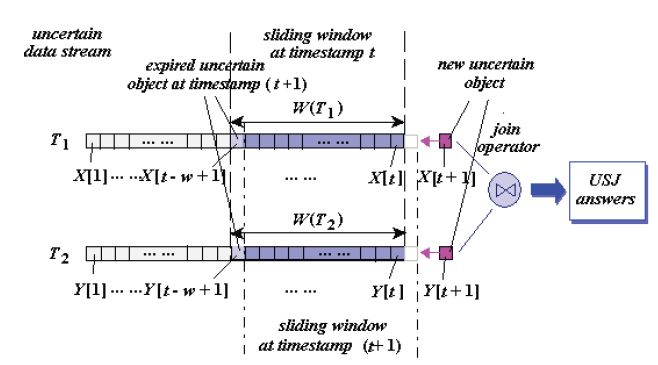
\includegraphics[scale=0.8]{figures/dataconnection.png}
	\centering
	\caption{Παράδειγμα ένταξης εικόνας από άλλο άρθρο ή βιβλίο (Πηγή: \cite{[ACC+03]})}
	\label{dataconnection}
\end{figure}

Στο κείμενό σας, πρέπει να παραθέσετε άρθρα, βιβλία, ιστοσελίδες, άλλες διπλωματικές κλπ. που διαβάσατε. Παραδείγματα παραπομπών:

* από βιβλία: \cite{[RSV02]}

* από άρθρα σε περιοδικά: \cite{[ACC+03],[DRS09],[GBE+00]}

* από άρθρα σε πρακτικά επιστημονικών συνεδρίων: \cite{[JMS+08],[MHP05],[PS11]}

* από ιστοσελίδες: \cite{[Ora11]}

* από διπλωματικές ή άλλες δημοσιευμένες εργασίες: \cite{[Pap15]}


\section{<Τίτλος για σχετική θεματική περιοχή 2>}

Γράψτε το κείμενό σας...

 % Include the second content chapter
%\chapter{Τεχνικές Προβλέψης Χρονοσειρών}
\label{chap3}

\section{Εισαγωγή}
Μέσα από την εφαρμογή των κλασικών μεθόδων προβλέψεων αποσκοπούμε με χρήση των παρελθοντικών παρατηρήσεων μιας χρονοσειράς να εκτιμήσουμε τις μελλοντικές.
Η πρόβλεψη αποτελεί μια πολυβηματική διαδικασία που θα αναπτυχθεί στο παρόν κεφάλαιο και περιγράφεται από το διάγραμμα ροής του Σχήματος \ref{classicmethodology}.

\begin{figure}[t!]
  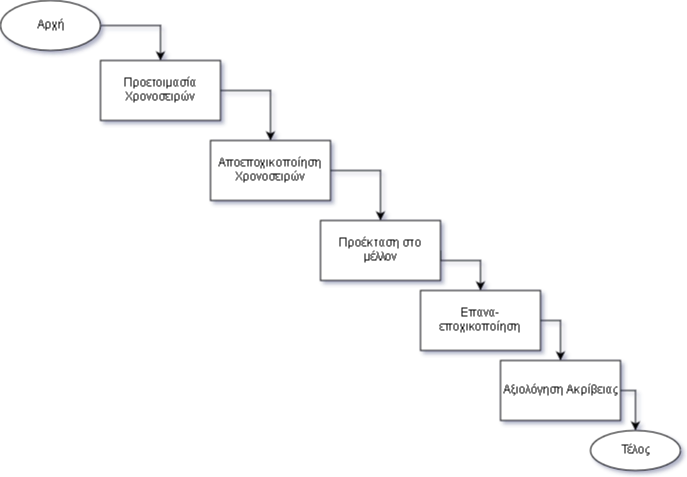
\includegraphics[scale=0.5]{figures/classicforecasting(1).png}
\centering
\caption{Κλασική μεθοδολογία πρόβλεψης χρονοσειρών}
\label{classicmethodology}
\end{figure} 



\section{Προετοιμασία Χρονοσειρών}

\subsection{Γραφική Αναπαράσταση Δεδομένων}
Κατά τη διαδικασία της επεξεργασίας και πρόβλεψης μιας χρονοσειράς είναι σημαντικό ο ερευνητής να μπορεί να αποκτήσει μία διαίσθηση πάνω στα δεδομένα. Μέσω της αναπαράστασης τους σε μια γραφική απεικόνιση μπορεί εύκολα να διαπιστώσει ποια ποιοτικά χαρακτηριστικά της χρονοσειράς έχουν έντονο βάρος. Μπορεί έτσι να εντοπίσει ότι η χρονοσειράς χαρακτηρίζεται από ακραίες τιμές, έχει έντονη τάση ή μοτίβα που επαναλαμβάνονται και εποχιακότητα.



\subsection{Διαχείριση Ιδιομορφίας Χρονοσειρών}
Είναι αρκετά σύνηθες τα δεδομένα που προορίζονται για πρόβλεψη να παρουσιάζουν δυσμορφίες. Μη σταθερή συχνότητα μεταξύ δύο συνεχόμενων τιμών μιας χρονοσειράς τη καθιστά αταίριαστη για πολλές από τις κλασικές μεθόδους πρόβλεψης. Τα δεδομένα βρίσκονται σε συχνότητα διαφορετική από αυτή που θέλουμε να προβλέψουμε, λόγου χάρη ημερήσια, ενώ είναι επιθυμητό να παραχθούν μηνιαίες προβλέψεις.
Επίσης, υπάρχει η περίπτωση ενώ εν γένει η σειρά αποτελείται από τιμές που ισαπέχουν μεταξύ τους στο πεδίο του χρόνου, παρουσιάζονται περιπτώσεις που δεν έχουν σημειωθεί κάποιες παρατηρήσεις. Αυτές τις ελλείψεις τις λέμε κενές τιμές. Μία άλλη ιδιομορφία που μπορεί να συναντήσουμε και καθιστά τη χρονοσειρά μη διαχειρίσιμη από αρκετές μεθόδους είναι η ύπαρξη μηδενικών τιμών. 

\subsubsection{Επαναδειγματοληψία}
Στη περίπτωση που το χρονικό διάστημα μεταξύ δύο παρατηρήσεων δεν είναι σταθερό ή ακόμα και διαφορετικό από αυτό που θέλουμε να έχουμε στη πρόβλεψή μας, πρέπει να φέρουμε τα δεδομένα μας σε μια πιο κανονικοποιημένη μορφή. Μία μέθοδος που μπορούμε να ακολουθήσουμε είναι η μέθοδος της επαναδειγματοληψίας (\en{resampling}). Η χρονοσειρά, συχνά, περιγράφει φαινόμενα συνεχούς χρόνου μέσα από διακριτό χρόνο. Με την επαναδειγματοληψία χρησιμοποιούμε τη πληροφορία που έχουμε ήδη στη διάθεση μας για να δημιουργήσουμε μια νέα χρονοσειρά που της έχουμε ορίσει τους ακριβείς χρόνους των παρατηρήσεων. Η επιλογή αυτή γίνεται τόσο βάσει των τιμών που ήδη έχουμε αλλά και του στόχου μας για το αποτέλεσμα στη πρόβλεψη.

Έχοντας επιλέξει τη νέα συχνότητα των δεδομένων, μένει να επιλέξουμε με ποιόν τρόπο θα γίνει η μετατροπή. Μπορούμε να διακρίνουμε δύο βασικές περιπτώσεις ανάλογα με το αν μεταβαίνουμε από μεγαλύτερη σε μικρότερη συχνότητα. Την δειγματοληψία προς τα πάνω \en{(upsampling)} και τη δειγματοληψία προς τα κάτω \en{(downsampling)}.

Για παράδειγμα, μπορούμε να έχουμε δεδομένα που έχουν συλλεχθεί σε ωριαία βάση, ενώ η πρόβλεψή μας θέλουμε να γίνει σε ημερήσιο επίπεδο. Τότε χρησιμοποιούμε \en{downsampling}, μετατρέποντας τα δεδομένα με μια κατάλληλη συνάρτηση, όπως το άθροισμα των ωριαίων τιμών, ο μέσος όρος τους, το μέγιστο ή το ελάχιστο. Αντίστοιχα αν τα δεδομένα μας θέλουμε να αλλάξουν από μικρότερη συχνότητα σε μεγαλύτερη, όπως από ημερήσια σε ωριαία, χρησιμοποιούμε \en{upsampling}, που συνδυάζεται συνήθως συμπληρώνοντας παρεμβολικά τις νέες χρονικές στιγμές που προκύπτουν. Η παρεμβολή θα περιγραφεί στη διαχείριση κενών τιμών

\subsubsection{Διαχείριση κενών τιμών}
Αρχικά, εφόσον αυτό είναι δυνατό, προσπαθούμε να βρούμε τις τιμές που μας λείπουν από άλλες πηγές, πέραν της αρχικής που λάβαμε τα δεδομένα. Επίσης, αν οι σειρές που αναλύουμε είναι λίγες στο πλήθος και γνωρίζουμε τη φύση της, μπορούμε να ορίσουμε απευθείας τις κενές τιμές, στη περίπτωση που βάσει των παραπάνω μπορούμε να κάνουμε μία ασφαλή εκτίμηση.

Στη πράξη τα παραπάνω δεν είναι συχνά εφικτά, ιδίως στις περιπτώσεις που πρέπει να γίνει διαχείριση μεγάλου αριθμού χρονοσειρών. Έτσι διακρίνουμε δύο περιπτώσεις: χρονοσειρές με εποχιακή συμπεριφορά και μη.

Όταν η χρονοσειρά προς επεξεργασία παρουσιάζει σαφή εποχιακή συμπεριφορά, μπορούμε να εκτιμήσουμε τη τιμή βάσει των τιμών των αντίστοιχων περιόδων με την εν λόγω κενή τιμή. Ένας τρόπος είναι να πάρουμε τον μέσο όρο. Έτσι, αν σε μία ετήσια χρονοσειρά με μηνιαία δεδομένα, αν μας λείπει η τιμή από κάποιον Ιανουάριο, μπορούμε να τη συμπληρώσουμε ως τον μέσο όρο των άλλων.

Στη περίπτωση που δε μιλάμε για εποχιακή συμπεριφορά, χρησιμοποιούμε τη μέθοδο της παρεμβολής για να συμπληρώσουμε τις κενές τιμές μας. Χρησιμοποιώντας τις γειτονικές τιμές μιας ακολουθίας κενών τιμών, τις συμπληρώνουμε με χρήση κατάλληλης μεθόδου. Μια κλασική προσέγγιση είναι να συμπληρωθούν γραμμικά, ως σημεία της ευθείας που ορίζουν οι δύο οριακές τιμές. Ειδάλλως μπορούμε να χρησιμοποιήσουμε άλλες μεθόδους όπως να δώσουμε τη τιμή της πιο κοντινής από τις δύο τιμές, να τις συμπληρώσουμε ως σημεία ενός πολυωνύμου δευτέρου, τρίτου ή μεγαλύτερου βαθμού. Πιο σύνθετες μέθοδοι είναι αυτές των \en{splines, krogh,} βαρυκεντρίκή και πολυωνυμική κατά σημείο.

\subsubsection{Διαχείριση μηδενικών τιμών}
Διακρίνουμε δύο περιπτώσεις, αν η παρατήρηση είναι πράγματι μηδενική ή έχει πάρει αυτή τη τιμή λόγω λάθους στη συλλογή δεδομένων. Προφανώς, στη δεύτερη περίπτωση χειριζόμαστε αυτές τιμές σαν να ήταν κενές και ακολουθούμε τις διαδικασίες που περιγράφηκαν προηγουμένως.

Αλλιώς, αν οι μηδενικές τιμές είναι λίγες, δεν θα επηρεάσουν σε μεγάλο βαθμό τα μοντέλα πρόβλεψης μας. Σε αντίθετη περίπτωση, χρησιμοποιούμε ειδικά μοντέλα για τη διαχείριση διακοπτόμενης ζήτησης.  

\subsection{Ημερολογιακές προσαρμογές}

Η χρονοσειρές είναι συχνό να περιγράφουν τιμές που σχετίζονται με ανθρώπινες ενέργειες και επηρεάζονται από τον τρόπο που είναι οργανωμένη η ανθρώπινη κοινωνία. Έτσι προετοιμάζοντας μια χρονοσειρά για πρόβλεψη πρέπει να εντοπίσουμε με πιο τρόπο συμβαίνει αυτή η επιρροή.

Σε ημερήσιες χρονοσειρές, αυτό γίνεται προσαρμόζοντας τα δεδομένα βάσει ημερολογιακών γεγονότων. Καθορίζουμε, λοιπόν, τις εργάσιμες μέρες συσχετισμένες με το μέγεθος που περιγράφει η σειρά και τις αντίστοιχες αργίες. Έχοντας προσδιορίσει τα παραπάνω, υπολογίζουμε τις εργάσιμες μέρες για κάθε περίοδο των δεδομένων μας ($N_t$) και τον μέσο όρο τους για όλες τις περιόδους ($N_{avg}$).

Μπορούμε έτσι να εξομαλύνουμε τη τιμή της κάθε παρατήρησης μας ως εξής:
\[ Y_t^{'} = Y_t . \frac{N_{avg}}{N_t} \]

\section{Προέκταση χρονοσειρών}

\subsection{Εισαγωγή}

Αφότου έχουμε προετοιμάσει τη χρονοσειρά και την έχουμε αποσυνθέσει στα επιμέρους της στοιχεία, όπως περιγράφηκε στο προηγούμενο κεφάλαιο, προχωράμε στην εφαρμογή κάποιου μοντέλου πρόβλεψης στα αποεποχικοποιημένα δεδομένα. Στόχος στην εφαρμογή του μοντέλου είναι το αποτέλεσμα που θα προκύψει να είναι όσο πιο ακριβές δύναται, δηλαδή οι τιμές που θα παράξει το μοντέλο να είναι όσο το δυνατόν πιο κοντά στις πραγματικές που θα έχουμε στη διάθεση μας με τη πάροδο του χρόνου. Στο παρόν κεφάλαιο θα μελετήσουμε τις στατιστικές μεθόδους πρόβλεψης.

\subsection{\en{Naive:} η αφελής μέθοδος}

H \en{Naive} είναι η πιο απλή μέθοδος στατιστικής πρόβλεψης. Θεωρεί ότι η τιμή που θα ακολουθήσει χρονικά ταυτίζεται με τη τιμή της παρούσας περιόδου, σύμφωνα με τη παρακάτω σχέση, όπου το $F_t$ είναι η πρόβλεψη κατά τη χρονική στιγμή $t$ και $Y_t$ η πραγματική τιμή της σειράς:
\[ F(t+1) = Y(t) \]

Είναι φυσικό ότι η \en{Naive} δεν παράγει ακριβείς προβλέψεις αλλά μπορούμε να τη χρησιμοποιήσουμε ως βάση σύγκρισης (\en{benchmark}) άλλων μεθόδων.

\subsection{Μοντέλα Παλινδρόμησης}

Η ανάλυση της παλινδρόμησης αποσκοπεί στην εύρεση συσχετίσεων μεταξύ μιας εξαρτημένης μεταβλητής και μίας ή περισσοτέρων ανεξάρτητων μεταβλητών. Έχει ευρεία χρήση στη διαδικασία των προβλέψεων, τόσο ως μοντέλο πρόβλεψης αλλά και ως υποβοήθημα σε άλλες μεθόδους, όπως θα δούμε παρακάτω. Κυρίως, όμως μας επιτρέπει να βγάλουμε συμπεράσματα για τη συσχέτιση της ανεξάρτητης μεταβλητής και των εξαρτημένων μεταβλητών.

\subsubsection{Απλή Γραμμική Παλινδρόμηση}

Η μέθοδος, που φέρει και το όνομα μέθοδος των ελαχίστων τετραγώνων, περιγράφει μία ευθεία με την ελάχιστη απόσταση ανά σημείο από τα πραγματικά δεδομένα. Για να τη λάβουμε πρέπει να ελαχιστοποιηθεί το άθροισμα σφαλμάτων στη δεύτερη εξίσωση που ακολουθεί. Επίσης, φαίνεται αναλυτικά πως προκύπτουν και οι συντελεστές:

\[\hat{Y_i} = \alpha + \beta X_i \]
\[ \sum{e_i^2} = \sum{(Y_i - \hat{Y_i})^2} \]
\[ \beta = \frac{ \frac{ \sum{X_i Y_i}}{n} - \bar{X} \bar{Y}} { \frac{\sum{X_i^2}}{n} - \bar{X}^2 } =  \frac{\sum{(X_i - \bar{X})(Y_i - \bar{Y})}} {\sum{(X_i - \bar{X})^2}} \]
\[ \alpha = \bar{Y} - \beta \bar{X} \]

Για να χρησιμοποιήσουμε τη μέθοδο της Απλής Γραμμικής Παλινδρόμησης, πρέπει να υπάρχει εξάρτηση της ανεξάρτητης μεταβλητής από τη τιμή ή τη μεταβολή κάποιας άλλης. Για να ελέγξουμε αν αυτό συμβαίνει, χρησιμοποιούμε τον συντελεστή γραμμικής συσχέτισης $r$ που αποτελεί έναν δείκτη του βαθμού που συσχετίζονται δύο μεταβλητές μεταξύ τους και για δύο μεταβλητές $X, Y$ προκύπτει ως εξής:

\[ {Cov}_{XY} = \frac{\sum{(X_i - \bar{X})(Y_i - \bar{Y})}}{n} \]
\[ {Cov}_{XX} = \frac{\sum{(X_i - \bar{X})^2}}{n} = {Var}_X = S_X^2 \]
\[ {Cov}_{YY} = \frac{\sum{(Y_i - \bar{Y})^2}}{n} = {Var}_Y = S_Y^2 \]


\[ r_{XY} = \frac{ {Cov}_{XY}} {\sqrt{{Cov}_{YY} *{Cov}_{XX} }} = \frac{ {Cov}_{XY} } { S_Y * S_X}
\]

Και προκύπτει ότι ο συντελεστής $r_{XY}$ λαμβάνει τιμές στο διάστημα από -1 έως 1.

Ο συντελεστής γραμμικής συσχέτισης επιδέχεται δύο ερμηνείες:

\begin{itemize}
    \item Μας δείχνει την κατεύθυνση της σχέσης μεταξύ των δύο μεταβλητών, δηλαδή αν όταν οι τιμές της μίας αυξάνονται, οι τιμές τις άλλης μειώνονται οι αυξάνονται. Επίσης, μπορεί να μας δείξει ότι η μεταβολές της μίας είναι ανεξάρτητες από τις άλλης.
    \item Μας δείχνει τον βαθμό συσχέτισης και συνεπώς τη δυνατότητα της γραμμής παλινδρόμησης να εκφράσει τη σχέση μεταξύ των μεταβλητών. Όσο το $r_{XY}$ πλησιάζει κατά απόλυτη τιμή τη μονάδα τόσο μικρότερη είναι η απόκλιση των πραγματικών τιμών της εξαρτημένης μεταβλητής από αυτές του μοντέλου.
\end{itemize}

Η μέθοδος των ελάχιστων τετραγώνων χρησιμοποιείται ως μοντέλο πρόβλεψης χρονοσειρών, απλά θέτοντας ως ανεξάρτητη μεταβλητή το χρόνο. Η γραμμή προκύπτει όπως περιγράψαμε προηγουμένως από τα ιστορικά δεδομένα, και προεκτείνοντας τη στο χρόνο λαμβάνουμε τις τιμές τις πρόβλεψης για τις χρονικές στιγμές που μας ενδιαφέρουν.

\subsubsection{Πολλαπλή Παλινδρόμηση}

Υπάρχουν περιπτώσεις που έχουμε πληροφορία για περισσότερες ανεξάρτητες μεταβλητές, τότε χρησιμοποιούμε τη μέθοδο της πολλαπλής παλινδρόμησης, η παίρνει την εξής μορφή:

\[ Y = \beta_0 + \beta_1 * X_1 + \beta_2 * X_2 + \dots + b_k * X_k + e \]

Αντίστοιχα με πριν, πρέπει να ελαχιστοποιηθεί το τετραγωνικό σφάλμα. Για να βρούμε τις τιμές των συντελεστών που μας οδηγούν στο ποθητό αποτέλεσμα, προσδιορίζουμε τις τιμές των μερικών παραγώγων της συνάρτησης του σφάλματος για κάθε συντελεστή. Κατόπιν λύνουμε το γραμμικό σύστημα που προκύπτει αν θέσουμε τη κάθε μερική παράγωγο ίση με το μηδέν. 




\subsection{Μοντέλα Εκθετικής Εξομάλυνσης}

Οι μέθοδοι εκθετικής εξομάλυνσης εμφανίστηκαν στο τέλος της δεκαετίας του 40', από τον \en{Brown} με σκοπό την πρόβλεψη αποθεμάτων και συνεχίζονται να εξελίσσονται ως σήμερα, αποτελώντας τις πιο δημοφιλείς μεθόδους προβλέψεων. Ο λόγος είναι ότι πρόκειται για σχετικά απλά μοντέλα με ευκολία χρήσης, μικρές υπολογιστικές απαιτήσεις και την δυνατότητα να παράξουν ακριβείς προβλέψεις ακόμα και με σχετικά μικρό ιστορικό παρατηρήσεων. Έτσι, χρησιμοποιούνται συχνά για τη παράλληλη πρόβλεψη πολλών χρονοσειρών, συνήθως με μικρό ορίζοντα πρόβλεψης. 

Σε όλα τα μοντέλα που ακολουθούν έχουμε μια εξομάλυνση των ιστορικών δεδομένων. Χρησιμοποιούνται συντελεστές βαρύτητας, που μειώνονται εκθετικά όσο πηγαίνουμε πίσω στο χρόνο, για να υπολογίσουμε τον μέσο όρο των παρατηρήσεων και να απαλλαχθούμε από τις τυχαίες διακυμάνσεις.

Προκύπτουν συνολικά 12 τύποι μοντέλων εξομάλυνσης ως συνδυασμός των παρακάτω:

\begin{itemize}
  \item Πρότυπα τάσης:

    \begin{itemize}
      \item Σταθερού Επιπέδου
      \item Γραμμικής Τάσης
      \item Εκθετικής Τάσης
      \item Φθίνουσας Τάσης
    \end{itemize}
  \item Πρότυπα εποχιακότητας:

    \begin{itemize}
      \item Άνευ Εποχιακότητας
      \item Προσθετικής Εποχιακότητας
      \item Πολλαπλασιαστικής Εποχιακότητας
    \end{itemize}
\end{itemize}

Ακολουθούν κάποια βασικά μοντέλα εκθετικής εξομάλυνσης.


\subsubsection{Απλή εκθετική εξομάλυνση}

Το μοντέλο της απλής εκθετικής εξομάλυνσης (\en{Simple Exponential Smoothing}) είναι ένα μοντέλο σταθερού επιπέδου που είναι ιδανικό για πρόβλεψη ενός βήματος. Επίσης, είναι κατάλληλο για χρονοσειρές που παρουσιάζουν υψηλό θόρυβο ή έντονο το στοιχείο της τυχαιότητας. Περιγράφεται από τις παρακάτω σχέσεις:
\[ e_t = Y_t - F_t \]
\[ S_t = S_{t-1} + \alpha * e_t \]
\[ F_{t+1} = S_t \]

Εκτός των $F_t$ και $Y_t$ που δηλώνουν τα ίδια μεγέθη όπως στη $Naive$, έχουμε το $e$ που δηλώνει το σφάλμα, το $S$ που δηλώνει το επίπεδο και το $\alpha$, τον συντελεστή εξομάλυνσης της μεθόδου με δυνατές τιμές ανάμεσα στο 0 και στο 1.
Βλέπουμε, λοιπόν, ότι πρέπει να χρησιμοποιήσουμε δύο παραμέτρους: τη πρώτη τιμή της πρόβλεψη $F_1$ και το παράγοντα εξομάλυνσης $\alpha$. Αν επιλέξουμε μεγάλη τιμή για το $\alpha$, η τελική τιμή της πρόβλεψης βασίζεται λιγότερο στις αρχικές τιμές και με $\alpha = 1$ η μέθοδος ταυτίζεται με τη \en{Naive}. Επίσης για χρονοσειρές πολύ μεγάλου μήκους η συνεισφορά της αρχικής πρόβλεψης στη τελική τιμή μειώνεται εκθετικά με το μήκος. 

Υπάρχουν διάφοροι τρόποι να ορίσουμε το αρχικό επίπεδο μια χρονοσειράς, μερικοί εκ των οποίων είναι:

\begin{itemize}
    \item Ο μέσος όρος όλων των τιμών της χρονοσειράς
    \item Ο μέσος όρος ν το πλήθος αρχικών τιμών της σειράς 
    \item Η πρώτη τιμή 
    \item Να υπολογίσουμε τη γραμμή της γραμμικής παλινδρόμησης και να θέσουμε το αρχικό επίπεδο ως το σταθερό επίπεδο αυτής της γραμμής
  \end{itemize}

Για να εντοπίσουμε τον κατάλληλο συντελεστή εξομάλυνσης για βέλτιστη ακρίβεια πρέπει να λάβουμε υπόψιν μας τόσο το θόρυβο της σειράς όσο και τη σταθερότητα του μέσου όρου της. Σε περίπτωση έντονου θορύβου, μικρή τιμή του συντελεστή μας διασφαλίζει ότι το μοντέλο μας δε θα αντιδρά υπερβολικά στο θόρυβο. Πρόσθετα, στη περίπτωση που μεταβάλλεται ο μέσος όρος των τιμών της σειράς όσο προχωράμε στο πεδίο του χρόνου, ένα μεγάλος συντελεστής εξομάλυνσης επιτρέπει στο μοντέλο να ακολουθεί αυτή τη μεταβολή. 


\subsubsection{Εκθετική εξομάλυνση γραμμικής τάσης}

Μια επέκταση της προηγούμενης μεθόδου είναι το μοντέλο εκθετικής εξομάλυνσης για γραμμικής τάση \en{Holt Exponential Smoothing} που εισήχθηκε από τον \en{Holt} το 1957. Η μέθοδος περιγράφεται από τις επόμενες εξισώσεις:

\[ e_t = Y_t - F_t \]
\[ S_t = S_{t-1} + T_{t-1} + \alpha * e_t \]
\[ T_t =  T_{t-1} + \alpha * \beta * e_t \]
\[ F_{t+m} = S_t + m * T_t \]

Όπου το νέο στοιχείο $T_t$ δηλώνει την τάση του μοντέλου κατά τη χρονική στιγμή $t$. Εδώ το $\alpha$ αποτελεί τον συντελεστή εξομάλυνσης του επιπέδου ενώ το $\beta$ το συντελεστή εξομάλυνσης της τάσης. Τόσο το αρχικό επίπεδο και η αρχική τάση πρέπει να προσδιοριστούν με προσοχή καθώς έχουν μεγάλη επιρροή στις τιμές του μοντέλου της πρόβλεψης. Για το πρώτο ακολουθούμε μία από τις μεθόδους υπολογισμού που περιγράφηκαν στην απλή εκθετική εξομάλυνση. Για την αρχική τάση μπορούμε να χρησιμοποιήσουμε μία από τις παρακάτω:

\begin{itemize}
    \item Διαφορά των δύο πρώτων τιμών της χρονοσειράς
    \item Διαφορά της τιμής μια παρατήρησης της χρονοσειράς με τη πρώτη, και διαίρεση του αποτελέσματος με τον αριθμό των χρονικών βημάτων που μεσολαβούν μεταξύ τους 
    \item Να υπολογίσουμε τη γραμμή της γραμμικής παλινδρόμησης και να θέσουμε την αρχική τάση ως τη κλίση αυτής της γραμμής
  \end{itemize}



\subsubsection{Μοντέλο μη γραμμική τάσης}

Το μοντέλο μη γραμμικής τάση εισήχθηκε το 1985 από τους \en{Gardner} και {McKenzie}, αφότου είχε παρατηρηθεί ότι το μοντέλο γραμμικής τάσης πολλές φορές παρουσίαζε θετική προκατάληψη, ειδικά όταν εφαρμοζόταν με στόχο μεσοπρόθεσμες ή μακροπρόθεσμες προβλέψεις. Το μοντέλο περιγράφεται από τις εξής σχέσεις:

\[ e_t = Y_t - F_t \]
\[ S_t = S_{t-1} + T_{t-1} + \alpha * e_t \]
\[ T_t =  T_{t-1} + \alpha * \beta * e_t \]
\[ F_{t+m} = S_t + \sum_{i=1}^{m}{\phi^{i}* T_t} \]

Παρατηρούμε ότι η αλλαγή σε σχέση με το προηγούμενο μοντέλο που περιγράψαμε εντοπίζεται στη τελευταία εξίσωση που, αντί να πολλαπλασιάζεται η τελευταία τάση που εντοπίσαμε με τη χρονική διαφορά σε περιόδους της τιμής προς πρόβλεψη από τη τελευταία τιμή των δεδομένων μας, έχουμε τη τελευταία τάση να πολλαπλασιάζεται με το άθροισμα των στοιχείων γεωμετρικής προόδου με λόγο ίσο με $\phi$ και μήκος $m$. Η παράμετρος $\phi$, που ονομάζεται παράμετρος διόρθωσης της τάσης, καθορίζει το μοντέλο ως εξής:

\begin{itemize}
\item Για $\phi = 0$, το μοντέλο ταυτίζεται με αυτό της απλής εκθετικής εξομάλυνσης
\item Για $0 < \phi < 1$, το μοντέλο χαρακτηρίζεται από φθίνουσα τάση
\item Για $\phi = 1$, το μοντέλο ταυτίζεται με το μοντέλο γραμμικής τάσης 
\item Για $\phi > 1$, έχουμε εκθετική εξομάλυνση με εκθετική τάση
\end{itemize}

Για να προσδιορίσουμε το αρχικό επίπεδο και την αρχική τάση, χρησιμοποιούμε τις μεθόδους που περιγράφηκαν στις προηγούμενες υποενότητες.


\subsection{Μέθοδος \en{Theta}}

Η μέθοδος Θ είναι μια μονοδιάστατη μέθοδος πρόβλεψης που εισήχθηκε από τον Ασημακόπουλο το 1999. Κατά το μοντέλο, η χρονοσειρά αναλύεται σε δύο ή περισσότερες χρονοσειρές ή αλλιώς γραμμές \en{Theta}. Κάθε μία από τις προκύπτουσες σειρές προβλέπεται ξεχωριστά, είτε με το ίδιο είτε με διαφορετικό μοντέλο πρόβλεψης, και η τελική πρόβλεψη είναι ο συνδυασμός των επιμέρους αποτελεσμάτων. 

Στην απλούστερη περίπτωση, το κλασσικό μοντέλο Θ, έχουμε δύο γραμμές \en{Theta}. Η πρώτη είναι μία ευθεία γραμμή που προκύπτει από την ευθεία γραμμικής παλινδρόμησης που μοντελοποιεί τα δεδομένα, η \en{Theta Line (0)}. Η δεύτερη, \en{Theta Line (2)} προκύπτει ως εξής:

\[ ThetaLine(2) = 2*Y - LRL\]

Όπου $Y$ η αρχική χρονοσειρά και $LRL$ η ευθεία που προκύπτει από τη μέθοδο ελαχίστων τετραγώνων. 

Η μέθοδος Θ βασίζεται στην μεταβολή των τοπικών καμπυλοτήτων μιας χρονοσειράς. Η μεταβολή αυτή λαμβάνει χώρα με τη χρήση της παραμέτρου θ που εφαρμόζεται στις δεύτερες διαφορές τις χρονοσειράς ως εξής: 

\[ Y_t^\theta = \theta*Y_t^{''} \]
\[ Y_t^{''} = Y_t - 2*Y_{t-1} + Y_{t-2} \]

Διακρίνουμε διαφορετικές συμπεριφορές των γραμμών Θ ανάλογα με τις τιμές τις παραμέτρου:
\begin{itemize}
    \item Αν $\theta=0$ η σειρά ταυτίζεται με την ευθεία γραμμικής παλινδρόμησης
    \item Αν $\theta=-1$ η σειρά που προκύπτει είναι η συμμετρική της αρχικής ως προς την ευθεία γραμμικής παλινδρόμησης
    \item Αν $\theta>1$ έχουμε πιο έντονες καμπυλότητες, ανάλογες του βαθμού της παραμέτρου
\end{itemize}

Το τελικό μοντέλο πρόβλεψης προκύπτει ως γραμμικός συνδυασμός των γραμμών Θ, έτσι ώστε τα βάρη της κάθε σειράς να αθροίζουν στο 1. Στην κλασσική μέθοδο, όπως είδαμε στην εξίσωση υπολογισμού της \en{Theta Line (2)}, έχουμε πάρει τα βάρη ίσα με 0.5 και για τις δύο γραμμές.

\section{Αξιολόγηση Προβλέψεων}

Αφότου έχουμε ολοκληρώσει τη διαδικασία πρόβλεψης πρέπει να αξιολογήσουμε κατά πόσο το μοντέλο μας παρήγαγε ακριβές προβλέψεις και στη περίπτωση που εφαρμόσαμε περισσότερα μοντέλα, πιο από αυτά είναι το πιο ακριβές. Για να το πετύχουμε αυτό χρησιμοποιούμε ένα σύνολο στατιστικών δεικτών αξιολόγησης της ακρίβειας. Αυτοί οι δείκτες, ή αλλιώς σφάλματα, μπορούν να χρησιμοποιηθούν για να μετρήσουν την απόδοση του υπό εφαρμογή μοντέλου στο σύνολο των δεδομένων του ιστορικού της χρονοσειράς, που είναι δηλαδή γνωστά στο μοντέλο μας (\en{in-sample error}, είναι στις τιμές του ορίζοντα πρόβλεψης (\en{out-of-sample error}). Αφότου ο σκοπός μας είναι να έχουμε ακριβή αποτύπωση της μελλοντικής εξέλιξης της χρονοσειράς, ενδιαφέρον για τη μέτρηση της απόδοσης του μοντέλου παρουσιάζει η δεύτερη κατηγορία. 

Γενικά ορίζουμε ως σφάλμα της πρόβλεψης μιας περιόδου:
\[e_i = Y_i - F_i\]

Το απλό ποσοστιαίο σφάλμα ως:
\[p_i = \frac{ 100 * e_i} { Y_i } (\%) \]

Επίσης, έχουμε το απλό σχετικό σφάλμα, που είναι ο λόγος του σφάλματος της υπό εξέταση μεθόδου σε σχέση με κάποια άλλη μέθοδο. Συνήθως η μέθοδος σύγκρισης είναι η \en{Naive}, που περιγράφηκε πρωτύτερα:

\[r_i = \frac{  e_i} { e_i^* } \]

Το απλό κανονικοποιημένο σφάλμα βρίσκεται από τη παρακάτω σχέση:

\[q_i = \frac{  e_i} { \frac{1}{n-1} \sum_{i=2}^n {|Y_i - Y_{i-1}|}} \]


Στον Πίνακα \ref{tab:errors} βλέπουμε τους πιο κοινούς δείκτες ακρίβειας. To \en{mean} υποδηλώνει τον αριθμητικό μέσο όρο, το \en{median} τη διάμεσο και το \en{gmean} το γεωμετρικό μέσο. Επίσης το \textbf{1} λαμβάνει τη τιμή 1 στη περίπτωση που αυτό που εσωκλείει είναι αληθές, αλλιώς παίρνει την τιμή 0.

\begin{table}[h]
\centering
\begin{tabular}{|c|>{\centering\arraybackslash}m{6cm}|c|}
  \hline
  \textbf{Συντομογραφία} & \textbf{Πλήρες Όνομα} & \textbf{Τύπος} \\
  \hline
  \en{ME }  &   \en{Mean Error}  & $mean(e_i)$ \\
  \en{MSE }  &   \en{Mean Squared Error}  & $mean(e_i^2)$ \\
  \en{RMSE }  &   \en{Rooted Mean Squared Error}  & $\sqrt{mean(e_i^2)}$ \\
  \en{MAE }  &   \en{Mean Absolute Error}  & $mean(|e_i|)$ \\
  \en{MdAE }  &   \en{Median Absolute Error}  & $median(|e_i|)$ \\
  \en{MAPE }  &   \en{Mean Absolute Percentage Error}  & $mean(|p_i|)$ \\
  \en{MdAPE }  &   \en{Median Absolute Percentage Error}  & $median(|p_i|)$ \\
  \en{sMAPE }  &   \en{Symmetric Mean Absolute Percentage Error}  & $mean(\frac{200*|Y_i - F_i|}{Y_i + F_i)})$ \\
  \en{sMdAPE }  &   \en{Symmetric Median Absolute Percentage Error}  & $median(\frac{200*|Y_i - F_i|}{Y_i + F_i)})$ \\
  \en{MRAE }  &   \en{Mean Relative Absolute Error}  & $mean(|r_i|)$ \\
  \en{MdRAE }  &   \en{Median Relative Absolute Error}  & $median(|r_i|)$ \\
  \en{GMRAE }  &   \en{Geometric Mean Relative Absolute Error}  & $gmean(|r_i|)$ \\
  \en{RelMAE }  &   \en{Relative Mean Absolute Error}  & $MAE/MAE_b$ \\
  \en{RelRMSE }  &   \en{Relative Mean Squared Error}  & $RMSE/RMSE_b$ \\
  \en{LMR }  &   \en{Log Mean Squared Error Ratio}  & $\log(RelMSE)$ \\
  \en{PB }  &   \en{Percentage Better}  & $100 * mean( \textbf{1}\{|r_i|<1\})$ \\
  \en{PB(MAE) }  &   \en{Percentage Better (MAE)}  & $100 * mean( \textbf{1}\{MAE<MAE_b\})$ \\
  \en{PB(MSE) }  &   \en{Percentage Better (MSE)}  & $100 * mean( \textbf{1}\{MSE<MSE_b\})$ \\
  \en{MAsE }  &   \en{Mean Absolute Scaled Error}  & $mean(|q_i|)$ \\
  \en{MdAsE }  &   \en{Median Absolute Scaled Error}  & $median(|q_i|)$ \\
  \hline
\end{tabular}
\caption{Δείκτες Ακρίβειας}
\label{tab:errors}
\end{table}


Στηριζόμενοι στη δουλειά των \en{Hyndman} και \en{Koehler} μπορούμε να χωρίσουμε τους δείκτες αυτούς στις εξής κατηγορίες:

\subsubsection{Δείκτες που εξαρτώνται από τη κλίμακα των δεδομένων}

Η κατηγορία αυτή αποτελείται από τους δείκτες \en{MSE, RMSE, MAE, MdAE} που συναρτώνται της απόλυτης τιμής των δεδομένων. Βοηθούν ιδιαίτερα όταν καλούμαστε να συγκρίνουμε την απόδοση διαφόρων μοντέλων πρόβλεψης επί της ίδιας χρονοσειράς. Σε περίπτωση που τους εφαρμόζουμε, όμως, σε ένα σύνολο χρονοσειρών με διαφορετική κλίμακα μπορούν να παράξουν αποπροσανατολιστικά αποτελέσματα. Το προτέρημα του δείκτη \en{RMSE} έναντι του απλού \en{MSE} είναι ότι μας δίνει μετρήσεις στην ίδια κλίμακα με αυτή της χρονοσειράς στην οποία εφαρμόζεται. Επίσης, οι δύο παραπάνω δείκτες είναι ιδιαίτερα ευαίσθητοι στις ακραίες τιμές μιας χρονοσειράς, σε σύγκριση με του \en{MAE, MdAE} λόγω του τετραγωνισμού του σφάλματος. Αυτό τους καθιστά ακατάλληλους για χρήση στην αξιολόγηση της ακρίβειας πρόβλεψης.

\subsubsection{Δείκτες που βασίζονται σε ποσοστιαία σφάλματα}

Σε αυτή την ομάδα, από τους δείκτες που είδαμε, ανήκουν οι \en{ MAPE, MdAPE, sMAPE} και \en{sMdAPE}. Οι δείκτες \en{MAPE} και \en{MdAPE} υστερούν στο γεγονός ότι δεν δύνανται να λάβουν τιμή όταν οι πραγματικές παρατηρήσεις είναι μηδενικές και επιπρόσθετα παρουσιάζουν έντονη ασυμμετρία όταν οι παρατηρήσεις είναι κοντά στο μηδέν. Έτσι, ο δείκτες \en{MAPE} παρουσιάζει χαρακτηριστικά μεγάλες τιμές σε σχέση με τον δείκτη \en{MdAPE}.  Μπορούμε, βέβαια, με τη χρήση λογαριθμικών μετασχηματισμών να προσδώσουμε μια σταθερότητα στους δείκτες. Επίσης, οι δύο αυτοί δείκτες δίνουν μεγαλύτερη βαρύτητα στα θετικά έναντι των αρνητικών σφαλμάτων. Αντίθετα, οι δείκτες \en{sMape} και \en{sMdAPE} δεν παρουσιάζουν στον ίδιο βαθμό το πρόβλημα των μηδενικών τιμών. Αν και το όνομα τους υποδηλώνει συμμετρία, έχουν το μειονέκτημα ότι οι αισιόδοξες και οι απαισιόδοξες προβλέψεις δεν υπολογίζονται με το ίδιο βάρος.

\subsubsection{Δείκτες σχετικών σφαλμάτων}

Από τους δείκτες που έχουμε εξετάσει οι \en{MRAE, MdRAE} και \en{GMRAE} ανήκουν σε αυτή την κατηγορία. Το πρόβλημα με αυτή των ομάδα δεικτών είναι ότι στις περιπτώσεις που το σφάλμα αναφοράς λαμβάνει αρκετά μικρές τιμές ο λόγος $r_i$ τείνει να έχει άπειρη διακύμανση.

\subsubsection{Σχετικοί δείκτες}

Το πλεονέκτημα των σχετικών δεικτών \en{RelMAE, RelRMSE} και \en{PB} είναι ότι αποφεύγουν το πρόβλημα που είδαμε στη προηγούμενη κατηγορία δεικτών με τις άπειρες τιμές. Επίσης, μας επιτρέπουν να αποφασίσουμε εύκολα πιο από τις μεθόδους που συγκρίνουμε είναι πιο ακριβής, ανάλογα με τον αν ο δείκτες έχει τιμή μεγαλύτερη της μονάδας. Βέβαια, καθότι απαιτούν αρκετές προβλέψεις δε μπορούμε να τους εφαρμόσουμε όταν έχουν πρόβλεψη με ορίζοντα ίσο με ένα. 

\subsubsection{Κανονικοποιημένοι δείκτες}

Οι κανονικοποιημένοι δείκτες \en{MAsE, MdAsE} προσφέρουν τόσο ευκολία στην ερμηνεία αντίστοιχη των σχετικών δεικτών, ενώ συγχρόνως μπορούν να εφαρμοστούν για μοναδική περίοδο πρόβλεψης. Επιπρόσθετα, είναι απαλλαγμένες από το επίπεδο της κάθε χρονοσειράς και εφαρμόσιμες σε μαζική πρόβλεψη χρονοσειρών, αποφεύγοντας τις απροσδιοριστίες των ποσοστιαίων σφαλμάτων.





 % Include the third content chapter

\backmatter

\chapterstyle{default} % Reset the chapter style back to the default used for non-content chapters

%----------------------------------------------------------------------------------------
%	BIBLIOGRAPHY
%----------------------------------------------------------------------------------------

\bibliographystyle{plainnat} % Use the plainnat bibliography style

\bibliography{bibliography} % Use the bibliography.bib file as the source of references

%----------------------------------------------------------------------------------------
%	INDEX
%----------------------------------------------------------------------------------------

\printindex % Print the index

%----------------------------------------------------------------------------------------

\end{document}